\section{集合的测量}
\label{sec:comb-set-measurement}
\label{sec:analysis-set-structures}

区间$[a,b]$的长度是$b-a$，但实轴上的集合未必是一个区间。
本节要解决的问题是：怎样把区间的长度推广到更一般的实数集合，并在原来的区间上仍得到$b-a$？
本章后面的积分需要这样的长度：把输入范围分成若干块后，只有知道各块的大小，才能按这些大小累计函数取值。
有限集合的元素个数与加权计数是另一类测量，可以先用它们说明为集合赋予大小时应遵守的相加规则。

集合的大小与点之间的距离是两种不同的结构。
在同一条实轴上使用同一种通常距离，既可以测量区间的长度，也可以数集合中的点；
因此，选定度量并不能唯一确定测度，即给集合赋予大小的方式。

本节先用有限集合的计数与加权计数说明相加规则，再从区间长度构造Jordan测量；有理点集将说明，只用有限个区间逼近还不够。
为此，随后利用可数集的列举规则改用可数覆盖，定义勒贝格外测度。
外测度对每个集合都有定义，却不保证不交部分精确相加，所以再用精确分割条件选出可测集，在可测集上得到可数可加的勒贝格测度。
最后推导勒贝格测度在集合列、零测集与几乎处处方面的性质，并用康托尔集说明零测集可以不可数。

\subsection{有限集与Jordan测量}
\label{sec:comb-counting-to-weight}

我们先把目标限制在有界的实数集合上，希望给这些集合建立与区间长度相容的测量方法。
例如$[0,1]\cup[2,3]$由两段互不重叠、长度各为$1$的区间组成，总长度应为$2$。
由这个例子可以看出所求测量应满足的一条规则：集合分成有限个两两不交的部分时，总量等于各部分测量值之和。

下面先在有限集合上用计数和加权计数说明这条规则，再回到实轴。
实轴上的长度将从区间出发：先计算有限个区间的并，再用这些简单集合从内、外两侧逼近更一般的有界集合；
只有当内部与外部的长度估计逼近同一个数时，才用这个数定义集合的Jordan测量。

\subsubsection{有限集的测量}

\paragraph{计数与加权计数}

在有限集合上，最直接的测量是数元素个数；若不同元素代表不同的份量，还可以给每个元素指定权重。
设$X=\{x_1,\ldots,x_m\}$中的点互异，每点带有非负权重$w_i$。
把落在$A\subseteq X$中的点的权重相加，定义
\[
 \mu(A)=\sum_{i:x_i\in A}w_i.
\]
所有$w_i=1$时，$\mu(A)=|A|$，即元素个数；改变权重时，元素不变，测量值却可以改变。
例如在$X=\{a,b\}$上给$a,b$分别指定权重$1,2$，就有$\mu(\{a\})=1$、$\mu(\{b\})=2$、$\mu(X)=3$。

若$A_1,\ldots,A_k$两两不交，并集中的每个点恰好落入其中一组，它的权重在等式两侧都只计一次，故
\[
 \mu\left(\bigcup_{j=1}^k A_j\right)=\sum_{j=1}^k\mu(A_j).
\]
这称为\term{有限可加性}（finite additivity）。它沿用计数的加法规则，
但相加的是各组的权重，不必是元素个数。

\paragraph{集合权重与函数值}

$\mu(A)$只测量集合$A$本身。后面还要在集合上累计函数取值，届时每个点的贡献等于函数值乘以该点的权重。
下面在同一个两点集合上比较等权与加权两种累计。
\begin{example}[两点集合上的等权与加权累计]
沿用$X=\{a,b\}$，给$a,b$分别指定权重$1,2$，并取函数值$f(a)=3$、$f(b)=-1$。

每点计$1$时，集合大小为$|X|=2$，函数的取值和为$f(a)+f(b)=3-1=2$。

按权重计时，集合大小为$\mu(X)=1+2=3$，函数的加权和为
\[
 3\cdot1+(-1)\cdot2=1.
\]
\end{example}

同一组元素和同一组函数值，在两种权重下给出不同的集合大小（$2$与$3$），也给出不同的累计值（$2$与$1$）。
表~\ref{tab:analysis-metric-measure-integral}汇总这些计算；本章后面的积分将把这种加权累计推广到更一般的集合与函数。
\begin{table}[htbp]
 \centering\small
 \begin{tabularx}{\linewidth}{@{}lXX@{}}
 \toprule
 考察对象 & 所用规则 & $X=\{a,b\}$上的结果\\
 \midrule
 元素个数 & 每点计$1$ & $|X|=2$\\
 集合权重 & $a,b$分别计$1,2$ & $\mu(X)=3$\\
 数值的等权累计 & 取值为$3,-1$ & $3-1=2$\\
 数值的加权累计 & 同一取值采用权重$1,2$ & $3-2=1$\\
 \bottomrule
 \end{tabularx}
 \caption{有限计数与加权累计。相同的元素范围和相同的数值取值仍可采用不同权重；只有先固定权重，累计值才有确定含义。}
 \label{tab:analysis-metric-measure-integral}
\end{table}

\paragraph{点数与长度}

有限集合的例子说明了不交部分如何相加，但每点计$1$的规则不能给出区间长度。
例如$[0,1]$和$[0,2]$都含有无限多个点，逐点计数都得到无穷，而它们的长度分别应为$1$和$2$。
所以，要推广区间长度，必须另行规定与几何长度相容的测量规则。

单点$[a,a]$的长度为$0$，有限个单点的并也应有长度$0$。
这与非退化区间的长度为正并不矛盾：非退化区间含无限多个点，不能写成有限个单点的并，所以有限可加性不适用于把它拆成全部单点的操作。
第~\ref{sec:analysis-countable-outer-measure}节讨论可数覆盖时还要用到另一事实：非退化区间的点也不能列成一个序列。

因此我们改以区间长度为起点：先计算能由有限个区间组成的集合的长度，再研究不能这样表示的集合。

\subsubsection{Jordan测量}

\paragraph{区间长度与初等集}

一个区间的长度由端点决定；有限个区间组成的集合，也可以先拆成互不重叠的小段再相加。
对端点为$a\leq b$的有界区间$I$，规定长度为$\ell(I)=b-a$，不因端点是否包含而改变；
单点与空集的长度为$0$。

为反复使用这类可以直接计算长度的集合，先给它们一个名称：
我们把有限个这样的区间的并称为\term{初等集}（elementary set），空集也约定为初等集。
例如$[0,1]\cup[2,3]$是初等集，两段长度相加得到$2$。
区间发生重叠时，需要先消除重复计算：$[0,2]\cup[1,3]=[0,3]$的长度为$3$，不能把原来两段的长度直接相加为$4$。

一个初等集$B$可以有多种区间表示，所以先按一种表示规定长度，再检查结果与表示无关。
取定一种表示，将其中所有端点排序，按相邻端点之间的开区间及端点本身切分，得到有限个两两不交的小段；把属于$B$的小段长度相加，记为$\ell(B)$。
若采用另一种表示，把两组端点合在一起排序，便得到两种切分的共同细分。
区间从$c$处分成两段时，$(c-a)+(b-c)=b-a$，所以细分不改变总长度。
因此，两种表示给出同一个$\ell(B)$。

对有限个初等集取它们端点的共同细分可知，初等集的并、交、差仍为初等集，不交初等集的长度有限可加。
一般的有限覆盖只给出不等式：若$B\subseteq\bigcup_{j=1}^k B_j$，则
$\ell(B)\leq\sum_{j=1}^k\ell(B_j)$，因为在共同细分下，$B$的每个小段在右侧至少计算一次，重叠的小段还会被重复计算。
特别地，取$k=1$可知$A\subseteq B$时$\ell(A)\leq\ell(B)$。

\paragraph{内容量与外容量}

初等集的长度已经可以计算，但有界集合只要求一个集合包含在某个有限区间内，并不要求它本身由有限个区间组成。
下面的倒数点集就是这样的集合。
\begin{example}[倒数点集不是初等集]
\label{ex:set-measure-reciprocal-not-elementary}
考虑
\[
 E=\{1,1/2,1/3,\ldots\}\subseteq[0,1].
\]
它包含于$[0,1]$，因此有界。

对任意$u>0$，$E\cap[u,1]$中的点$1/n$都满足$n\leq1/u$，所以这一部分只有有限多个点。

由此可知$E$不包含任何正长度区间。假如$E$包含端点为$c<d$的区间，由$E\subseteq(0,1]$可知$c\geq0$；
取$u=(c+d)/2>0$，区间中的$[u,d)$便落在$E\cap[u,1]$中。它含无限多个点，与上一步的有限性矛盾。

若$E$是初等集，组成它的每个区间都包含于$E$，只能是单点或空集，于是$E$只有有限多个点；这与$E$含无限多个点矛盾。
所以$E$不是初等集。
\end{example}

因此初等集的长度公式不能直接用于$E$。
为了测量$E$这样的集合，一种办法是保留初等集作为计算工具，用包含关系给出长度估计。
把初等集$A$放在$E$内部，即$A\subseteq E$，$\ell(A)$就应是$E$的长度的下界；
用初等集$B$包住$E$，即$E\subseteq B$，$\ell(B)$就应是上界。
我们希望内部估计尽可能大、外部估计尽可能小，因此分别取内部长度的上确界与外部长度的下确界。
这两个数未必相等；若相等，内部与外部的估计就共同确定了一个长度值，可以把它作为$E$的测量值。

下面给这两个界命名，并按它们是否相等规定哪些有界集合可以用这种方法测量；两侧的候选都是初等集，长度都按初等集的长度$\ell$计算。
\begin{definition}[Jordan内容量与外容量]
\label{def:analysis-jordan-content}
对有界集合$E\subseteq\mathbb R$，定义\term{Jordan内容量}（Jordan inner content）与\term{Jordan外容量}（Jordan outer content）为
\[
 \begin{aligned}
 j_*(E)&=\sup\{\ell(A):A\subseteq E,\ A\text{为初等集}\},\\
 j^*(E)&=\inf\{\ell(B):E\subseteq B,\ B\text{为初等集}\}.
 \end{aligned}
\]
若$j_*(E)=j^*(E)$，称$E$为Jordan可测集，二者的共同值记为$j(E)$，称为它的\term{Jordan测量}（Jordan measure）值。
\end{definition}

对有界集合$E$，有界性保证外部候选非空且长度有限，空集则是内部候选；
又由$A\subseteq E\subseteq B$和初等集长度的单调性得$\ell(A)\leq\ell(B)$。所以
$0\leq j_*(E)\leq j^*(E)<\infty$。
上下确界一般不要求由某个最佳初等集取得；若$E$本身是初等集，内外都可以取$E$，结合$\ell(A)\leq\ell(E)\leq\ell(B)$便得$j_*(E)=j^*(E)=\ell(E)$。
所以新的定义保留了区间长度与有限区间并的长度，有限点集的测量值也仍为$0$。

倒数点集虽然不是初等集，它的两个容量却可以直接算出。
\begin{example}[倒数点集的Jordan测量为零]
\label{ex:set-measure-reciprocal-jordan-null}
仍取$E=\{1/n:n\geq1\}$。

内部：示例~\ref{ex:set-measure-reciprocal-not-elementary}已说明$E$不含正长度区间，所以包含于$E$的初等集只能由有限个单点组成，长度为$0$。于是
\[
 j_*(E)=0.
\]

外部：对每个整数$N\geq2$，取
\[
 B_N=\{1,1/2,\ldots,1/(N-1)\}\cup[0,1/N].
\]
前$N-1$个点分别由单点覆盖，其余的点$1/n$（$n\geq N$）全部落在$[0,1/N]$内，故$E\subseteq B_N$。
$B_N$是初等集，有限个单点不增加长度，所以$\ell(B_N)=1/N$。
于是$0\leq j^*(E)\leq1/N$对所有$N\geq2$成立，从而
\[
 j^*(E)=0.
\]

内外容量相等，所以$E$是Jordan可测集，且$j(E)=0$。
\end{example}

这个不属于初等集的无限点集仍然Jordan可测。
它的测量值来自有限逼近：外部候选的长度$1/N$可以任意小，内部候选的长度始终为$0$。

\paragraph{有限逼近与可加性}

内外数值相等也可以改写成误差条件：$E$为Jordan可测集，当且仅当对每个$\varepsilon>0$，
存在初等集$A\subseteq E\subseteq B$，使$\ell(B)-\ell(A)<\varepsilon$。
若$E$可测，按上确界和下确界的定义，各选一个与共同值$j(E)$相差小于$\varepsilon/2$的内部候选和外部候选即可。
反过来，若对每个$\varepsilon$都有这样的$A,B$，则$\ell(A)\leq j_*(E)\leq j^*(E)\leq\ell(B)$，两个容量之差小于任意正数，只能相等。

这个误差条件还保证有限次集合运算保持Jordan可测性。
分别以$A_E\subseteq E\subseteq B_E$和$A_F\subseteq F\subseteq B_F$夹住两个Jordan可测集，
它们的并夹在$A_E\cup A_F$与$B_E\cup B_F$之间，且
\[
 (B_E\cup B_F)\setminus(A_E\cup A_F)\subseteq(B_E\setminus A_E)\cup(B_F\setminus A_F).
\]
初等集$A\subseteq B$时，有限可加性给出$\ell(B)-\ell(A)=\ell(B\setminus A)$；再用有限覆盖不等式，新上下界的长度差不超过原来两份误差之和。

交集夹在$A_E\cap A_F$与$B_E\cap B_F$之间，差集$E\setminus F$夹在$A_E\setminus B_F$与$B_E\setminus A_F$之间。
两种情形中，外部逼近与内部逼近之差同样包含于$(B_E\setminus A_E)\cup(B_F\setminus A_F)$。
因此，Jordan可测集的有限并、交、差仍Jordan可测。

若$E,F$还不交，内部逼近$A_E,A_F$也不交。左端用不交初等集的有限可加性，右端用有限覆盖不等式，得到
\[
 \ell(A_E)+\ell(A_F)
 \leq j_*(E\cup F)\leq j^*(E\cup F)
 \leq\ell(B_E)+\ell(B_F).
\]
让各份逼近误差趋于零，两端都趋于$j(E)+j(F)$，所以$j(E\cup F)=j(E)+j(F)$。
这就是Jordan测量的有限可加性。论证中只合并了有限份逼近误差，所以它不能直接推广到无限多个集合的并。

\subsubsection{Jordan测量的局限}

\paragraph{有理点集的内外容量}

倒数点集$E$虽然不是初等集，仍能用有限区间并把外部长度压到任意小。
这是否意味着每个有界集合都能这样处理？下面考察$Q_0=\mathbb Q\cap[0,1]$，它将说明Jordan方法使用的有限逼近不能处理任意的有界集合。

先看$Q_0$在区间中的分布：任意非退化实区间$(a,b)$（$a<b$）都含有理数和无理数。
找有理数时，取正整数$q>1/(b-a)$，使相邻分数$p/q$与$(p+1)/q$的间距$1/q$小于区间长度。
令$p$为满足$p>aq$的最小整数，则$(p-1)/q\leq a<p/q$，于是$p/q\leq a+1/q<b$，即$p/q\in(a,b)$。

找无理数时，对区间内的有理数$r$，取正整数$k$使$\sqrt2/k<b-r$，则$r+\sqrt2/k$位于$(r,b)$内；
它若是有理数，$\sqrt2=k\bigl((r+\sqrt2/k)-r\bigr)$也将是有理数，矛盾。
所以$Q_0$和它在$[0,1]$内的补集都与$[0,1]$的每个正长度子区间相交。

利用这种分布，可以算出$Q_0$的两个容量。
\begin{example}[有理点集不Jordan可测]
\label{ex:set-measure-rationals-not-jordan}
设$Q_0=\mathbb Q\cap[0,1]$。

内部：任何正长度区间都含无理数，不可能完全落在$Q_0$中。
包含于$Q_0$的初等集因此只能由有限个单点组成，长度为$0$，所以
\[
 j_*(Q_0)=0.
\]

外部：设初等集$B$包含$Q_0$。把组成$B$的有限个区间的端点补齐，得到闭包$\overline B$；
补上有限个点不改变长度，所以$\ell(\overline B)=\ell(B)$。
若$[0,1]$内某点$x$不在$\overline B$中，由于$\overline B$是闭集，$x$附近就有一小段开区间完全避开$\overline B$，从而也避开$B$。
这段开区间在$[0,1]$内的部分仍有正长度，因而含有有理数，与$Q_0\subseteq B$矛盾。
因此$[0,1]\subseteq\overline B$，从而$\ell(B)=\ell(\overline B)\geq1$。
又因为$[0,1]$本身就是一个外部候选，得到
\[
 j^*(Q_0)=1.
\]

两个容量相差$1$，所以$Q_0$不Jordan可测。
\end{example}

\paragraph{有限覆盖的限制}

$Q_0$不Jordan可测（示例~\ref{ex:set-measure-rationals-not-jordan}），原因不在于有限覆盖中的区间还不够多。
无论选一百个还是一百万个区间，只要仍是有限个，它们的并就是初等集，例中的论证仍迫使任何覆盖$Q_0$的总长度至少为$1$。
倒数点集的情形不同：它可以把除有限个点以外的全部点装进靠近零的一个短区间；
有理点集却在$[0,1]$的每一小段中都出现，不能用一个越来越短的区间收拢剩下的点。

要突破这个下界，需要扩大允许使用的覆盖，而不是继续增加一次有限覆盖中的区间数。
如果能将$Q_0$列为$q_1,q_2,\ldots$，就可以给每个点分别安排一个开区间，
并把长度依次限制为$\varepsilon/2,\varepsilon/4,\varepsilon/8,\ldots$。
这样每个点都会被覆盖，总长度又由几何级数控制在$\varepsilon$以内，而$\varepsilon$可以任意小。
这里需要一整列区间共同覆盖全部点，其中任意有限前段本身都未必覆盖$Q_0$。

图~\ref{fig:measure-countable-cover}对比了两种覆盖规则；右侧的前四项只展示长度如何分配，并未单独完成对全部有理点的覆盖。

\begin{figure*}[htbp]
 \centering
 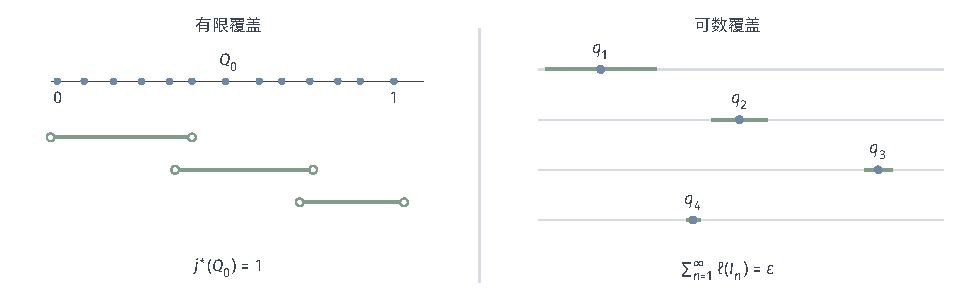
\includegraphics[width=169mm]{figures/00-shared/mathematical-preliminaries-upper/03-calculus/tikz/measure-countable-cover/figure.pdf}
 \caption{有限覆盖与可数覆盖。左侧画出一个有限开区间覆盖示例；对$Q_0=\mathbb Q\cap[0,1]$的任意有限区间覆盖，总长度均不小于$1$。右侧将一次完整覆盖改为可数个区间，图中取$\varepsilon=0.8$，只画列举中前四个点及其区间，长度依次为$\varepsilon2^{-n}$；使用全部区间时覆盖全部有理点，总长度为$\varepsilon$，并可随$\varepsilon$任意减小。点的有限示意不能表示有理点的完整稠密分布。}
 \label{fig:measure-countable-cover}
\end{figure*}

由此得到新的做法：允许用可数个区间组成一次完整覆盖，再用非负级数计算总长度。
实施这一做法需要第~\ref{sec:comb-countable-sets}节建立的列举与合并规则；下一小节从这些规则出发，定义新的外部长度估计。

\subsection{可数集与勒贝格外测度}
\label{sec:analysis-countable-outer-measure}

有限覆盖的限制已经说明了改变构造的理由：既要让每个可列举的点都分到自己的小区间，又要把所有区间的总长度控制住。
可数覆盖能同时做到这两件事，因为区间带有自然数编号，长度可以用已经学过的非负级数相加。

这一做法要用于后面的推导，还需要两项工具：可数个可数集合的并仍可数，保证合并若干组覆盖后仍是允许的覆盖；
非负双重级数可以合并，保证按组计算与统一编号计算得到同一个总长度。
这些工具建立后，就能定义勒贝格外测度，并检查它既能改进有理点集的估计，又保留普通区间的长度。

\subsubsection{可数覆盖的编号与长度}

第~\ref{sec:comb-countable-sets}节已定义可数集，并用对角列举证明自然数对、有理数与可数个可数集的并都可数。
因此$Q_0=\mathbb Q\cap[0,1]$可以列为$q_1,q_2,\ldots$，每个点都能分到自己的小区间；
合并一列可数覆盖时，所有区间也仍可统一编号。
余下要检查的是总长度：改变非负项的列举方式，不能改变覆盖长度的总和。

\paragraph{非负双重级数的合并}

沿用第~\ref{sec:analysis-continuous-limits}节对非负项级数规定的扩展总和，对$a_n\in[0,\infty]$有
\begin{equation}
 \sum_{n=1}^{\infty}a_n
 =\sup_{N\geq1}\sum_{n=1}^Na_n\in[0,\infty].
 \label{eq:comb-nonnegative-sum-supremum}
\end{equation}
非负性使有限和随加入新项而不减，所以也可以对所有有限索引集取上确界，结果相同。

对$a_{n,j}\geq0$，将双指标按任一无遗漏、无重复的顺序列成一个序列；由上一句，它的总和总是
\[
 S=\sup_{F\subseteq\mathbb N_+^2,\,F\text{有限}}
          \sum_{(n,j)\in F}a_{n,j},
\]
与所选顺序无关。下面证明$S=\sum_n\sum_j a_{n,j}$，即$S$等于先对每一行求和、再把各行之和相加的结果。

一方面，任取有限索引集$F$，它只涉及有限多行，并在每一行中只取有限多项；
每行取出的部分不超过该行之和，所以$\sum_{(n,j)\in F}a_{n,j}\leq\sum_n\sum_ja_{n,j}$。对$F$取上确界，得$S\leq\sum_n\sum_ja_{n,j}$。

另一方面，固定行数$N$与任意$\varepsilon>0$。若前$N$行之和都有限，对每个$n\leq N$选有限列数$J_n$，
使该行前$J_n$项之和超过整行之和减去$\varepsilon/N$。这些项组成一个有限索引集，所以
$S\geq\sum_{n=1}^N\sum_ja_{n,j}-\varepsilon$。令$\varepsilon\downarrow0$，再对$N$取上确界，得到$S\geq\sum_n\sum_ja_{n,j}$。
若某行之和为无穷，它的有限部分和可以超过任意给定的有限上界，同样迫使$S=+\infty$，此时两侧都为无穷。

这个证明只用到有限和与上确界的性质，因此这里的非负项换序不必借助后文的积分换序定理。

\subsubsection{勒贝格外测度}
\label{sec:comb-length-and-lebesgue-measure}

\paragraph{可数区间覆盖}

由于$Q_0$可以列为$q_1,q_2,\ldots$，逐点安排小区间的方案可以实施。
我们把这种覆盖方式用于一般集合：对$E\subseteq\mathbb R$，若有限或可数个有界开区间$I_j=(a_j,b_j)$满足$E\subseteq\bigcup_j I_j$，就称它们为$E$的可数区间覆盖。
区间可以重叠，也可以伸出$E$；它们的总长度为非负级数$\sum_j(b_j-a_j)$，允许等于$+\infty$。

“可数”限制的是覆盖区间的个数，不是$E$中的点数；一个开区间就可以覆盖含有不可数多个点的闭区间。
选择可数覆盖，是为了能逐项分配误差、用级数累计长度，并在合并覆盖时保留这两种能力。
前面没有给任意不可数族定义总长度，因此这里也不把“可数”放宽为不受限制的任意区间族。
采用开区间，则是为了在证明中使用闭区间的有限子覆盖性质；下面将用它保证原来的区间长度不被改变。

\paragraph{勒贝格外测度的定义}

一次覆盖可能伸出集合，也可能重复覆盖某些位置，所以它的总长度只是一个依赖于区间选择的外部估计。
为了尽量排除这些额外长度，我们对所有允许覆盖的总长度取下确界，得到勒贝格外测度。
\begin{definition}[勒贝格外测度]
\label{def:analysis-lebesgue-outer-measure}
对$E\subseteq\mathbb R$，定义其\term{勒贝格外测度}（Lebesgue outer measure）为
\begin{equation}
 m^*(E)=\inf\left\{\sum_{j=1}^{\infty}(b_j-a_j):
 \begin{array}{l}
 E\subseteq\bigcup_{j=1}^{\infty}(a_j,b_j),\\
 -\infty<a_j<b_j<\infty
 \end{array}\right\}.
 \label{eq:comb-lebesgue-outer-measure}
\end{equation}
这里也允许有限覆盖以及空集的空覆盖；空和为$0$。
\end{definition}

任意集合都能由覆盖整条实轴的一列区间覆盖，所以候选始终非空。
下确界可以为无穷，也不必由某个覆盖达到。
例如单点可以被任意短的开区间覆盖，其外测度为$0$；但任何覆盖都至少含一个非空开区间，总长度为正，所以没有覆盖能达到这个下确界。

\paragraph{空集与单调性}

空覆盖表明$m^*(\varnothing)=0$。
若$E\subseteq F$，任何覆盖$F$的区间族也覆盖$E$，
所以$F$的每个候选也是$E$的候选；在更大的候选集合上取下确界，结果不会更大，便得$m^*(E)\leq m^*(F)$。
这称为外测度的单调性，依据是两组候选覆盖之间的包含关系。

\paragraph{区间的外测度}

允许可数覆盖后，候选更多，下确界可能下降。我们希望有理点集的估计下降，但也必须检查普通区间的长度没有因此改变。
\begin{lemma}[区间的外测度等于长度]
\label{lem:set-measure-interval-outer-measure}
设$a<b$。对端点为$a,b$的有界区间$I$（两端可含可不含），有$m^*(I)=b-a$；无界区间的外测度为$+\infty$。
\end{lemma}
\begin{proof}
先证明$m^*([a,b])=b-a$。

上界：对任意$\varepsilon>0$，单个开区间$(a-\varepsilon/2,b+\varepsilon/2)$覆盖$[a,b]$，长度为$b-a+\varepsilon$。
令$\varepsilon\downarrow0$，得$m^*([a,b])\leq b-a$。

下界：这一侧必须控制每一种可数覆盖，不能只考察某一组区间。
任取$[a,b]$的可数开区间覆盖$\{(a_j,b_j)\}$。由闭区间的有限子覆盖性质（定理~\ref{thm:analysis-interval-finite-subcover}），其中有限个区间已经覆盖$[a,b]$；记它们的索引集为$F$。
初等集的有限覆盖不等式给出
\[
 b-a\leq\sum_{j\in F}(b_j-a_j)\leq\sum_{j=1}^{\infty}(b_j-a_j).
\]
对所有可数覆盖取下确界，得$m^*([a,b])\geq b-a$。

其他有界区间$I$包含长度任意接近$b-a$的闭区间，又有$I\subseteq[a,b]$，由单调性夹逼得$m^*(I)=b-a$。
无界区间包含任意长的有界闭区间，所以外测度为$+\infty$。
\end{proof}

所以改用可数覆盖后，区间的长度保持原值。

\paragraph{可数点集的外测度}

现在回到推动构造的例子，检验可数覆盖是否真正突破了有限覆盖的限制。
\begin{example}[可数点集的外测度为零]
\label{ex:set-measure-countable-outer-null}
设$E=\{x_1,x_2,\ldots\}$可数。任给$\varepsilon>0$，对每个$n$取
\[
 I_n=\bigl(x_n-\varepsilon2^{-n-1},\ x_n+\varepsilon2^{-n-1}\bigr).
\]
每个点$x_n$都落入$I_n$，所以这列区间覆盖全部$E$，且$\ell(I_n)=\varepsilon2^{-n}$。
于是
\[
 0\leq m^*(E)\leq\sum_{n=1}^{\infty}\varepsilon2^{-n}=\varepsilon.
\]
由于$\varepsilon$任意，$m^*(E)=0$。有限集只需用前有限个区间，同样得到外测度为$0$。
\end{example}

例中每个覆盖区间的长度都为正；趋于零的是整组覆盖的总长度上界，而不是一些未定义的正“无穷小”之和。

特别地，$m^*(Q_0)=0$，尽管$Q_0$的Jordan外容量为$1$。
有限覆盖的总长度不能低于$1$，可数覆盖却能把总长度压到任意给定的正数以内；改变的是一次完整覆盖所允许使用的区间族。
这与$m^*([0,1])=1$也不矛盾：$Q_0$可数，能够逐点编号；整个区间却不可数，无法给其中全部点各分配一个自然数编号，例中的覆盖方式不能用于$[0,1]$。

$m^*(Q_0)=0$回答的是外部估计能否下降的问题。
到这里，每个集合都已有外测度值，但还没有证明不交集合的外测度能够精确相加；要把外测度用于分块累计，还需要下面的可加性与可测性。

\subsubsection{可数可加性}

\paragraph{可数可加性的要求}

新的覆盖方式已经能累计可数个区间的长度，我们也希望测量规则能处理可数次不交分割。
例如，若一个可数点集作为各个单点的不交并参与精确相加，它的总长度就应等于单点长度之和。

一般地，对一个给集合赋值的映射$\nu$，希望有
\[
 \nu\left(\bigcup_{n=1}^{\infty}E_n\right)=\sum_{n=1}^{\infty}\nu(E_n),
 \qquad E_i\cap E_j=\varnothing\ (i\neq j),
\]
其中并集与各部分都应在$\nu$的赋值范围内。
这称为\term{可数可加性}（countable additivity），右侧是已经定义的非负项级数。

区间不可数，所以这一要求不允许把区间拆成全部单点后当作可数级数求和；
单点外测度为零与区间外测度为正并不矛盾。

\paragraph{外测度的可数次可加性}

已经建立的覆盖构造能先保证一个较弱的结论：把每个集合的覆盖合并，就得到并集的覆盖，
所以并集的外测度不超过各部分外测度之和。这只是不等式，并且不要求各集合不交。
这项性质称为\term{可数次可加性}（countable subadditivity）；名称中的“次”表示这里保证的是上界，不是精确相等。

每个集合未必有达到外测度的最优覆盖，证明时只能选近似最优覆盖。
因此需要把第$n$组的误差限制为$\varepsilon2^{-n}$，使合并无穷多组后总误差仍不超过$\varepsilon$。
\begin{theorem}[勒贝格外测度的可数次可加性]
\label{thm:analysis-outer-subadditivity}
对任意$E_1,E_2,\ldots\subseteq\mathbb R$，有
\begin{equation}
 m^*\left(\bigcup_{n=1}^{\infty}E_n\right)
 \leq\sum_{n=1}^{\infty}m^*(E_n).
 \label{eq:analysis-outer-subadditivity}
\end{equation}
\end{theorem}
\begin{proof}
若右侧为$+\infty$，不等式直接成立。
设右侧有限，则每个$m^*(E_n)$有限。给定$\varepsilon>0$，由下确界定义，
为每个$E_n$选择覆盖$\{I_{n,j}:j\geq1\}$，使
\[
 E_n\subseteq\bigcup_j I_{n,j},\qquad
 \sum_j\ell(I_{n,j})<m^*(E_n)+\varepsilon2^{-n}.
\]
空集可以取空覆盖，有限覆盖直接作为有限组处理。
所有$I_{n,j}$覆盖$\bigcup_nE_n$；可数个可数集的并仍可数，故它们是允许使用的一组覆盖。
再由非负双重级数的合并规则，
\[
 \begin{aligned}
 m^*\left(\bigcup_nE_n\right)
 &\leq\sum_{n,j}\ell(I_{n,j})\\
 &=\sum_n\sum_j\ell(I_{n,j})
 \leq\sum_nm^*(E_n)+\varepsilon.
 \end{aligned}
\]
最后让$\varepsilon\downarrow0$，得到所需不等式。
\end{proof}

\paragraph{一般外测度}

刚才的证明只给出不等式，尚未要求不交集合的值精确相加。
空集取值为零、单调性与可数次可加性这三条性质不依赖区间长度的具体形式；把它们抽取出来，便得到可用于其他测量构造的一般概念。
\begin{definition}[外测度]
\label{def:analysis-outer-measure}
集合$X$上的映射$\mu^*:\mathcal P(X)\to[0,\infty]$，若满足
\[
 \begin{gathered}
 \mu^*(\varnothing)=0,\\
 A\subseteq B\Longrightarrow\mu^*(A)\leq\mu^*(B),\\
 \mu^*\left(\bigcup_{n=1}^{\infty}E_n\right)\leq\sum_{n=1}^{\infty}\mu^*(E_n)
 \quad(E_n\subseteq X),
 \end{gathered}
\]
则称为\term{外测度}（outer measure）。
\end{definition}
前面已经证明勒贝格外测度满足这三条，所以它是外测度的一个实例；其中第三条来自覆盖的合并，而覆盖合并没有给出反向不等式。
即使$E_n$两两不交，分别覆盖它们的开区间也可能彼此重叠；集合不交并不会使覆盖的长度自动精确相加。
反过来，把覆盖并集的区间按任意集合切开，所得部分又未必是区间，不能直接沿用区间长度公式来分配总量。
因此，不能仅凭这三个条件便把式~\eqref{eq:analysis-outer-subadditivity}中的不等号改为等号。

下一步要补上的，是集合与这套外部估计之间的分割相容性：用一个集合切分任意测试集，切分后两部分的外测度之和仍等于原值。
我们将把满足这个要求的集合选出来，再证明在它们组成的范围内，不交可数并确实能够精确相加。

\subsection{可测集与勒贝格测度}
\label{sec:analysis-lebesgue-measurable-construction}

现在需要区分两个问题：一个集合能否取得外测度值，以及它能否在分割计算中保持精确相加。
第一个问题已经解决，任意集合都有$m^*$值；第二个问题还没有由覆盖构造保证。
要为积分准备可以反复分块的测量规则，就需要找出能够保持精确分割的集合，这就是引入可测集的原因。

下面保留原来的$m^*$数值，要求一个集合用来切分任何测试集时，都不改变分割前后的总量。
我们先写出这个条件，再证明满足条件的集合对取补和可数并封闭，最后证明限制到这一范围的$m^*$具有可数可加性。

\subsubsection{可测性的要求}

\paragraph{精确分割}

固定一个待检验的集合$A$，再任取测试集$E$。$A$把$E$分成落在$A$内的部分和落在$A$外的部分：
\[
 E=(E\cap A)\cup(E\setminus A),\qquad
 (E\cap A)\cap(E\setminus A)=\varnothing.
\]
次可加性已经保证$m^*(E)\leq m^*(E\cap A)+m^*(E\setminus A)$。
若要分割不改变总量，还需要反向不等式；缺少它时，两部分分别作外部估计，所得总和可能比整体的外部估计大。

外测度的三条公理确实不能自动排除这种情况，下面的两点空间就是一个有限例子。
\begin{example}[两点空间上不可加的外测度]
\label{ex:set-measure-two-point-outer-measure}
在两点集合$X=\{a,b\}$上，令$\mu^*(\varnothing)=0$，并令每个非空子集的值都为$1$。

单调性：若$A\subseteq B$且$A$非空，则$B$也非空，两者的值都为$1$；若$A$为空集，则$\mu^*(A)=0\leq\mu^*(B)$。

可数次可加性：若一列子集的并为空，各项都是空集，两侧均为$0$；若并非空，至少有一项非空，右侧至少为$1$，不小于左侧的$1$。

所以$\mu^*$是外测度。但取$E=X$、$A=\{a\}$时，
\[
 1=\mu^*(X)<\mu^*(\{a\})+\mu^*(\{b\})=2,
\]
即集合$\{a\}$不能精确分割测试集$X$。
\end{example}

这个例子只说明仅有三条公理不足以推出精确相加，并不是勒贝格外测度下的不可测集构造。
图~\ref{fig:measure-exact-splitting}把它与区间的精确分割放在一起，展示可测性条件要排除的总量变化。

\begin{figure*}[htbp]
 \centering
 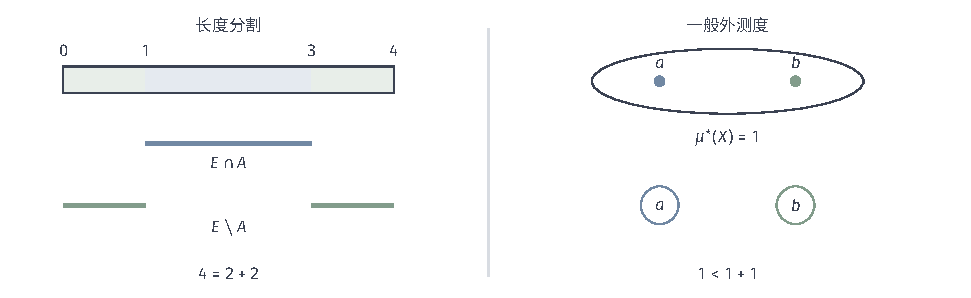
\includegraphics[width=169mm]{figures/00-shared/mathematical-preliminaries-upper/03-calculus/tikz/measure-exact-splitting/figure.pdf}
 \caption{精确分割与一般外测度的差别。左侧用$A=[1,3]$分割测试集$E=[0,4]$，落在$A$内的长度为$2$，外部两段总长度也为$2$，两者恢复原来的$4$；有限端点不改变长度。右侧使用正文两点空间的外测度，整体值为$1$，拆成两个单点后的值之和为$2$。右侧并非勒贝格不可测集的图像；左侧也只画了一个测试集，可测性定义要求对每个测试集都有精确等式。}
 \label{fig:measure-exact-splitting}
\end{figure*}

勒贝格外测度也存在不能保持精确分割的集合；这类不可测集的存在与构造可参考测度论教材\scite{math-hunter2011measure,math-folland1999real}，这里不展开。
下面直接以精确分割为条件选取可测集，并证明这类集合上的可加性。

\paragraph{可测集的定义}

我们希望$A$能够在不同范围的计算中反复参与分割，因此条件不能只针对某个预先选好的$E$，而要对所有测试集成立。
满足这一要求的$A$称为勒贝格可测集。
\begin{definition}[勒贝格可测集]
\label{def:analysis-lebesgue-measurable-set}
集合$A\subseteq\mathbb R$称为\term{勒贝格可测集}（Lebesgue measurable set），若对每个$E\subseteq\mathbb R$都有
\begin{equation}
 m^*(E)=m^*(E\cap A)+m^*(E\setminus A).
 \label{eq:comb-caratheodory-measurability}
\end{equation}
全体勒贝格可测集组成的集合族记为$\mathcal L(\mathbb R)$。
\end{definition}

式~\eqref{eq:comb-caratheodory-measurability}称为Carathéodory可测性条件。
由于$m^*(E)\leq m^*(E\cap A)+m^*(E\setminus A)$已由次可加性保证，验证可测性只需证明
$m^*(E)\geq m^*(E\cap A)+m^*(E\setminus A)$。
条件必须对每个$E$检验：只令$E=A$得到的是$m^*(A)=m^*(A)+m^*(\varnothing)$，对任意集合都成立，无法区分哪些分割与外测度相容。
“可测”并不表示此前无法给$A$求值；$m^*(A)$对任意$A$都已定义，新增的要求是$A$与所有测试集的分割相容。

外测度为零的集合不需要逐个验证分割；下面的引理一次处理所有这样的集合及其子集，以后处理零测余量和完备性时都会用到。
\begin{lemma}[零外测度集的子集可测]
\label{lem:analysis-zero-outer-measure-measurable}
若$N\subseteq\mathbb R$且$m^*(N)=0$，则每个$D\subseteq N$都勒贝格可测，并且$m^*(D)=0$。
\end{lemma}
\begin{proof}
单调性先给出$m^*(D)=0$。对任意测试集$E$，有
\[
 m^*(E\cap D)+m^*(E\setminus D)=0+m^*(E\setminus D)\leq m^*(E).
\]
结合外测度次可加性给出的反向不等式，得到可测性所需的精确分割等式。
\end{proof}

由示例~\ref{ex:set-measure-countable-outer-null}，$m^*(Q_0)=0$，所以此引理立即说明$Q_0$勒贝格可测。
利用$Q_0$的可测性，还可以算出$[0,1]$中无理点集的外测度。
\begin{example}[单位区间中无理点的外测度]
\label{ex:set-measure-irrationals-outer-measure}
在$Q_0$的可测性条件中取测试集$E=[0,1]$。由于$E\cap Q_0=Q_0$、$E\setminus Q_0=[0,1]\setminus Q_0$，得到
\[
 1=m^*([0,1])=m^*(Q_0)+m^*([0,1]\setminus Q_0)=0+m^*([0,1]\setminus Q_0).
\]
所以$[0,1]$中无理点组成的集合外测度为$1$。
\end{example}

有理点与无理点都分布在$[0,1]$的每一小段中，却不因此占有相同的长度。
可测性由分割等式判断，而不是由集合看起来是否稠密、光滑或规则判断。

\subsubsection{可测集族}

前面的定义逐个检验一个集合能否精确切分任意测试集。接下来还要检验：可测集经过取补、合并等运算后，是否仍然可测？

如果每次分块或合并都可能离开允许测量的范围，就无法反复使用这套测量方法。
Jordan测量就有这个问题：每个单点$\{q_n\}$都Jordan可测，它们的可数并$Q_0$却不Jordan可测（示例~\ref{ex:set-measure-rationals-not-jordan}）。
可见，每个部分都能参与测量，还不能保证合并后的对象也能参与测量。

勒贝格构造需要解决这个范围问题：先证明可测集族对所需运算封闭，再讨论合并后数值怎样相加。

\paragraph{取补与有限并}

取补对应保留分割的另一侧，有限并对应把有限块合为一块；先检查这两类操作，便能处理有限次分块计算。
下面始终用任意测试集$E$检验所得集合，并以已经证明的次可加性作为其中一个方向。

空集满足$m^*(E)=0+m^*(E)$，所以可测。
把$A$换成$\mathbb R\setminus A$只交换式~\eqref{eq:comb-caratheodory-measurability}右边的两项，因此取补保持可测，特别地$\mathbb R$也可测。

若$A,B$可测，先用$A$分割$E$，再用$B$分割$E\setminus A$，得到
\[
 \begin{aligned}
 m^*(E)&=m^*(E\cap A)+m^*((E\setminus A)\cap B)\\
 &\quad +m^*(E\setminus(A\cup B))\\
 &\geq m^*(E\cap(A\cup B))+m^*(E\setminus(A\cup B)).
 \end{aligned}
\]
前两部分恰好组成$E\cap(A\cup B)$，次可加性使它们的外测度之和不小于这个并的外测度，这就给出最后一行的不等式。
结合次可加性给出的另一方向，每个$E$都满足精确分割，所以$A\cup B$可测。
再由$A\cap B=(A^c\cup B^c)^c$和$A\setminus B=A\cap B^c$，得到有限交与差的可测性，这里的补集均相对于$\mathbb R$。

若$A,B$还不交，用$A$分割测试集$E\cap(A\cup B)$，又得到
\[
 m^*(E\cap(A\cup B))=m^*(E\cap A)+m^*(E\cap B).
\]
反复应用即可处理任意有限个两两不交的可测集。
这里同时得到了两件事：有限并仍在可测范围内；对不交的有限部分，切分前后的外测度精确相加。
后面处理可数并时，将从这两条有限结论出发，不预先假定无限情形已经成立。

\paragraph{可数并}

有限次合并不会离开可测范围，但一列集合的并不能在有限步内完成，所以可数并的可测性需要单独证明。
证明的办法是先精确切出前$N$块，再让非负部分和随$N$增加，而不直接调用尚未建立的测度可数可加性。

先设$C_n$两两不交且可测，令$U_N=\bigcup_{n=1}^NC_n$、$U=\bigcup_{n=1}^{\infty}C_n$。
对每个测试集$E$和每个$N$，先用可测集$U_N$分割$E$，再对$E\cap U_N$反复使用不交有限部分的等式，得到下式中的等号；
又因为$E\setminus U\subseteq E\setminus U_N$，外测度的单调性给出不等号：
\[
 \begin{aligned}
 m^*(E)
 &=\sum_{n=1}^Nm^*(E\cap C_n)+m^*(E\setminus U_N)\\
 &\geq\sum_{n=1}^Nm^*(E\cap C_n)+m^*(E\setminus U).
 \end{aligned}
\]
左侧不依赖$N$，令$N\to\infty$，非负部分和递增到级数之和，得到整列分割的下界；再用外测度的可数次可加性合并各个$E\cap C_n$，得到
\[
 m^*(E)\geq\sum_{n=1}^{\infty}m^*(E\cap C_n)+m^*(E\setminus U)
 \geq m^*(E\cap U)+m^*(E\setminus U).
\]
这就是$U$的可测性条件，故不交可测集的可数并可测。

若$A_n$不一定不交，令$C_1=A_1$、$C_n=A_n\setminus\bigcup_{j<n}A_j$。
每个$C_n$只用有限并与差集构成，所以已知可测；逐项去掉此前出现的部分，又使它们两两不交且并集不变。
对$C_n$应用刚才的结论，就证明了一般可数并仍可测。
至此，取补、有限并和可数并都不会使我们离开$\mathcal L(\mathbb R)$。

\paragraph{$\sigma$代数}

刚才证明的封闭性质，正是后续反复分块和合并时需要的范围保证。
为了在其他对象集合上也使用同样的保证，下面把“包含全集、取补封闭、可数并封闭”统一定义为$\sigma$代数。
\begin{definition}[$\sigma$代数]
\label{def:analysis-sigma-algebra}
设$X$为集合。若子集族$\mathcal A\subseteq\mathcal P(X)$满足
\[
 \begin{gathered}
 X\in\mathcal A,\\
 A\in\mathcal A\Longrightarrow X\setminus A\in\mathcal A,\\
 A_1,A_2,\ldots\in\mathcal A
 \Longrightarrow\bigcup_{n=1}^{\infty}A_n\in\mathcal A,
 \end{gathered}
\]
则称$\mathcal A$为$X$上的\term{$\sigma$代数}（sigma-algebra）。
\end{definition}

由取补可得$\varnothing\in\mathcal A$；在有限个集合之后补上无穷多个空集，便由可数并得到有限并。
De Morgan公式又给出可数交：$\bigcap_nA_n=X\setminus\bigcup_n(X\setminus A_n)$。
可数交在构造中经常出现：例如$\{a\}=\bigcap_{n\geq1}(a-1/n,a+1/n)$，单点就是一列开区间的交。
只对有限运算封闭的集合族不能保证这类由无限过程得到的集合仍在范围内，$\sigma$代数则把可数运算也纳入同一个范围。

在当前的勒贝格构造中，$\mathcal L(\mathbb R)$先由精确分割条件选出，再由前面的推导证明是$\sigma$代数；
我们没有预先假定所有可测集合自动具有这些封闭性。
在抽象测量问题中，则可以先指定一个$\sigma$代数来规定允许测量的范围。
两种做法的起点不同，但得到的范围具有相同的结构。

$\sigma$代数记录允许测量的子集，并保证这些子集经过所需的集合运算后仍在这一范围内；它没有给集合赋予大小，也没有单独保证任何数值的可加性。
所以接下来还要把已经构造的外测度放到这个可测范围上，证明它确实满足精确相加的规则。

\subsubsection{勒贝格测度}

\paragraph{限制外测度}

现在有了两个对象：$m^*$负责给集合赋值，$\mathcal L(\mathbb R)$负责保证取补和可数合并后仍在可测范围内。
我们保留$m^*$在可测集上的原值，把允许的输入从所有子集收缩为$\mathcal L(\mathbb R)$，并给这个限制后的赋值命名。
\begin{definition}[勒贝格测度]
\label{def:analysis-lebesgue-measure}
勒贝格外测度在$\mathcal L(\mathbb R)$上的限制
\[
 m:\mathcal L(\mathbb R)\to[0,\infty],\qquad m(A)=m^*(A),
\]
称为\term{勒贝格测度}（Lebesgue measure）。
\end{definition}

这一步没有重新计算任何可测集的大小：例如$m(Q_0)=m^*(Q_0)=0$，空集仍有$m(\varnothing)=0$。
改变的只是赋值的定义域；$m$在这个定义域上是否可数可加，还需要下面证明。

\paragraph{不交可测并的可数可加性}

$\sigma$代数已经保证可数并是允许的输入，因此等式左侧有定义；精确分割条件则使每个有限不交部分和都成为并集测量值的下界。
对这些下界取上确界，再结合外测度原有的次可加上界，就能把不等式收紧为等式。
\begin{theorem}[勒贝格测度的可数可加性]
\label{thm:analysis-lebesgue-countable-additivity}
若$A_n\in\mathcal L(\mathbb R)$两两不交，则
\[
 m\left(\bigcup_{n=1}^{\infty}A_n\right)=\sum_{n=1}^{\infty}m(A_n).
\]
\end{theorem}
\begin{proof}
记$A=\bigcup_n A_n$。前面已证明$A$可测；对每个$N$，由单调性与有限分割，
\[
 m(A)\geq m\left(\bigcup_{n=1}^NA_n\right)=\sum_{n=1}^Nm(A_n).
\]
对$N$取上确界，得到$m(A)\geq\sum_n m(A_n)$。
反向不等式正是外测度的可数次可加性，因为$m$与$m^*$在这些集合上相同。
\end{proof}

因此，从$m^*$到$m$经过了两个相接的步骤：先由精确分割条件选出$\mathcal L(\mathbb R)$，并证明它对可数并封闭，保证合并后的集合仍可测量；
再证明保留在这一范围上的数值可数可加，保证合并后集合的测量值等于不交部分之和。
这两步共同使勒贝格测度能够用于反复的分块累计。

类似构造也适用于一般外测度；这里只给出一维长度所需的关键封闭性与可加性步骤，
更一般的表述在\BookChapterRef{chap:measure-spaces}{第~\ref{chap:measure-spaces}章}建立，也可参考测度论教材\scite{math-hunter2011measure,math-folland1999real}。

\paragraph{区间与常见可测集}

可数可加性定理只适用于已经可测的集合，所以还要确认普通区间、开集等常用对象确实属于$\mathcal L(\mathbb R)$。
先从半直线开始：它只在一个位置切分区间，容易把可测性条件还原为已知的长度之和。

固定$t\in\mathbb R$，考虑半直线$H=(-\infty,t]$。
若$m^*(E)<\infty$，给定$\varepsilon>0$，选择总长度小于$m^*(E)+\varepsilon$的开区间覆盖$\{I_j\}$。
将每个$I_j$在$t$处切成$I_j\cap H$与$I_j\setminus H$两段；两段可能是开区间、半开区间或空集，
由引理~\ref{lem:set-measure-interval-outer-measure}，它们的外测度等于各自长度，而两段长度之和仍是$\ell(I_j)$。
两组小段分别覆盖$E\cap H$和$E\setminus H$，由外测度的次可加性得
\[
 \begin{aligned}
 &m^*(E\cap H)+m^*(E\setminus H)\\
 &\quad\leq\sum_j\bigl[m^*(I_j\cap H)+m^*(I_j\setminus H)\bigr]\\
 &\quad=\sum_j\ell(I_j)<m^*(E)+\varepsilon.
 \end{aligned}
\]
令$\varepsilon\downarrow0$就得到所需的反向不等式。
若$m^*(E)=\infty$，次可加性已迫使分割后的总和也为无穷，等式自动成立。
所以$H$可测。

半直线的差给出半开区间；再取可数并与可数交，就得到其他端点型式的区间和单点。
任意开集是其中所有有理端点开区间的并：对开集中的每个点，先取完全落在开集内的小区间，再利用有理数的稠密性缩小端点，使端点为有理数而区间仍含该点。
有理端点对可数，所以这是一组可数并；于是开集、其补集以及再经可数集合运算所得的集合都可测。
区间长度结论也随之保留为
\[
 m((a,b))=m([a,b])=m([a,b))=b-a,\qquad m(\{a\})=0.
\]

\paragraph{Borel集合}

区间与开集已经可测，但以后往往从它们出发反复取补、作可数并或可数交。
为了统一指明这些操作必然产生的集合，下面定义包含全部开区间的最小$\sigma$代数。

这样的最小范围确实存在：$\mathcal P(\mathbb R)$是一个包含所有开区间的$\sigma$代数，故候选不空。
把全部候选取交，所得集合族仍包含全集；对它的成员取补或作可数并，结果仍属于每个候选，所以交族本身也是$\sigma$代数。
它包含所有开区间，又包含于每个候选，因而正是所需的最小范围，称为由开区间生成的$\sigma$代数。
\begin{definition}[Borel $\sigma$代数]
\label{def:analysis-borel-sigma-algebra}
实轴上由所有开区间$(a,b)$（$a<b$）生成的最小$\sigma$代数记为$\mathcal B(\mathbb R)$，称为\term{Borel $\sigma$代数}（Borel sigma-algebra）。
对$X\subseteq\mathbb R$，令
\[
 \mathcal B(X)=\{X\cap B:B\in\mathcal B(\mathbb R)\},
\]
称为$X$上的Borel $\sigma$代数；其中的集合称为Borel集合。
\end{definition}

由前面对开集的表示，$\mathcal B(\mathbb R)$也等于所有开集生成的$\sigma$代数。
例如$\{a\}=\bigcap_{n\geq1}(a-1/n,a+1/n)$是Borel集合，可数点集作为可数个单点的并也是Borel集合。
各范围之间有
\[
 \mathcal B(\mathbb R)\subseteq\mathcal L(\mathbb R)\subseteq\mathcal P(\mathbb R),
 \qquad m=m^*\big|_{\mathcal L(\mathbb R)}.
\]
第一个包含关系来自可测范围的封闭性：$\mathcal L(\mathbb R)$已经是包含所有开区间的$\sigma$代数，必包含最小的$\mathcal B(\mathbb R)$。
第二个包含关系只说明可测集也是实轴子集，并不表示全部子集都可测；前面已经指出勒贝格外测度下存在不可测集，其构造不在这里展开。
这里$\mathcal B(\mathbb R)$与$\mathcal L(\mathbb R)$都是集合族，规定允许的范围；$m$与$m^*$是给集合赋值的函数，职责不同。

\paragraph{Jordan测量与勒贝格测度}

前面已经说明区间长度保持不变，现在进一步检验：每个Jordan可测集是否都勒贝格可测，且两种测量值相同。
证明中的零测余量由引理~\ref{lem:analysis-zero-outer-measure-measurable}处理：外测度为零的集合的任意子集都已可测，因此内部Borel部分之外的零测误差不会破坏可测性。

若$E$为Jordan可测集，对每个$n$取初等集$A_n\subseteq E\subseteq B_n$，
使$\ell(B_n)-\ell(A_n)<2^{-n}$。
令$A=\bigcup_nA_n$、$B=\bigcap_nB_n$，则$A,B$均为Borel集合，且$A\subseteq E\subseteq B$。
由于$B\setminus A\subseteq B_n\setminus A_n$，而在初等集上$m$与$\ell$相同，有
$m(B\setminus A)\leq\ell(B_n)-\ell(A_n)<2^{-n}$对所有$n$成立，故$m(B\setminus A)=0$。
$E\setminus A$包含于$B\setminus A$，由该引理可测，于是$E=A\cup(E\setminus A)$也可测。

最后比较数值。任一内部候选$A'\subseteq E$与外部候选$B'\supseteq E$都满足$\ell(A')=m(A')\leq m(E)\leq m(B')=\ell(B')$，
分别取上确界与下确界得$j_*(E)\leq m(E)\leq j^*(E)$，从而$m(E)=j(E)$。

因此Jordan可测集都勒贝格可测，数值保持一致；$Q_0$则说明逆向不成立：它在每个小区间中都稠密，不Jordan可测，却是可数Borel集合，勒贝格测度为零。

\subsection{勒贝格测度的性质}
\label{sec:comb-measurable-sets-and-weights}

勒贝格测度已经在可测集族$\mathcal L(\mathbb R)$上定义，并满足可数可加性。
积分要按可测集合的大小累计函数取值，计算中还会遇到包含、重叠以及逐步扩大或缩小的集合；
函数也可能只在长度为零的范围内取不同值。下面只就实轴上的勒贝格测度$m$，推导后面积分要用到的三组性质：
由不交分割得到的大小比较与集合列极限，零测集与几乎处处的例外语言，以及康托尔集与康托尔函数，前者说明零测集可以不可数，后者的全部增长集中在一个零测集上。
把这些结构推广到一般集合上的测度空间，留给\BookChapterRef{chap:measure-spaces}{第~\ref{chap:measure-spaces}章}。

\subsubsection{基本性质与集合列}
\label{sec:comb-set-approximation}
\label{sec:analysis-set-measure-continuity}

可数可加性只直接规定了不交可数并的测度。包含、重叠和嵌套的集合关系都要先改写成不交分割，才能使用这一规则。
下面先由分割得到大小比较和重叠集合的上界，再研究一列集合的并、交与测量值极限的关系。
以下集合均属于$\mathcal L(\mathbb R)$；推导只用到可数可加性与可测集族对取补、可数并的封闭性。

\paragraph{单调性}

若$A\subseteq B$，较大的集合只比$A$多出$B\setminus A$这一部分。对可测的$A,B$，差集也可测，且$A$与$B\setminus A$不交，因此
\[
 m(B)=m(A)+m(B\setminus A)\geq m(A).
\]
这称为测度的单调性：包含关系给出测量值的大小比较。

若$m(B)<\infty$，还可以写成$m(B\setminus A)=m(B)-m(A)$，用总量减去已知部分计算余量。
这里的有限性不能省略：可加等式允许无穷值，相减却不能出现$\infty-\infty$。
例如$A=(0,\infty)$、$B=\mathbb R$时两者的测度都为无穷，差集$(-\infty,0]$的测度不能由相减得到。

\paragraph{次可加性}

集合有重叠时，直接相加会重复计算。对可测集合列$A_n$，把每一步已经出现的部分去掉，令
\[
 B_1=A_1,\qquad B_n=A_n\setminus\bigcup_{j<n}A_j\quad(n\geq2).
\]
$B_n$仍可测、两两不交，且与原集合列有相同的并；又有$B_n\subseteq A_n$，故
\[
 m\left(\bigcup_nA_n\right)=\sum_nm(B_n)\leq\sum_nm(A_n).
\]
这就是可数次可加性：即使各部分有重叠，也能用各部分测度之和控制并集的测度。
它还说明可数个零测集的并仍是零测集，因为此时右侧为$0$；后面合并例外范围时会用到这一点。

若$A,B$的测度有限，还可以精确校正重复部分。把$A\cup B$分成两两不交的$A\setminus B$、$A\cap B$与$B\setminus A$，由可加性有
\[
 m(A)=m(A\setminus B)+m(A\cap B),\qquad m(B)=m(B\setminus A)+m(A\cap B),
\]
而$m(A\cup B)$等于三部分测度之和。前两式相加后减去一份$m(A\cap B)$，得到
\[
 m(A\cup B)=m(A)+m(B)-m(A\cap B).
\]
这是测度形式的容斥公式；有限性保证其中的减法有意义。
例如$A=[0,2]$、$B=[1,3]$时，右侧为$2+2-1=3$，正是$A\cup B=[0,3]$的长度。

\paragraph{递增集合列}

有时一个范围是逐步加入新部分形成的，例如用越来越多的区间逼近一个开集。此时要知道，每一步的测量值能否确定最终并集的测量值。
若$A_1\subseteq A_2\subseteq\cdots$且$A=\bigcup_nA_n$，记为$A_n\uparrow A$。
可测范围对可数并封闭，所以$A$可测；下面说明测量值也能取极限。

增量$B_1=A_1$、$B_n=A_n\setminus A_{n-1}$两两不交，且
$A_n=\bigcup_{j=1}^nB_j$、$A=\bigcup_{j=1}^{\infty}B_j$。
于是可数可加性把集合的逐步增加转成非负部分和的逐步增加：$m(A_n)=\sum_{j=1}^nm(B_j)$，$m(A)=\sum_{j=1}^{\infty}m(B_j)$，得到
\begin{equation}
 m(A)=\sup_{n\geq1}m(A_n)=\lim_{n\to\infty}m(A_n).
 \label{eq:comb-measure-continuity-below}
\end{equation}
这个结论称为测度的下连续性，不要求$m(A)$有限；非负部分和的极限也可以是$+\infty$。
例如$A_n=(0,1-1/n)$递增，并集为$(0,1)$，各步长度$1-1/n$趋于$1$，正好等于并集的长度。

\paragraph{递减集合列}

逐步去掉部分时，最终留下的是交集。若$A_1\supseteq A_2\supseteq\cdots$且$A=\bigcap_nA_n$，记为$A_n\downarrow A$。
交集可测，但要由各步测度恢复交集测度，还需要一个有限总量作为相减的起点。

设$m(A_1)<\infty$。把留下的范围改为已经去掉的范围，$A_1\setminus A_n$便递增到$A_1\setminus A$。
对它应用下连续性，再利用所有集合都包含在有限测度的$A_1$中，把差集的测度写成相减，得到
\[
 m(A_1)-m(A)=\lim_{n\to\infty}\bigl[m(A_1)-m(A_n)\bigr].
\]
所有减法都在有限数值之间进行，整理后有
\begin{equation}
 m(A)=\inf_{n\geq1}m(A_n)=\lim_{n\to\infty}m(A_n).
 \label{eq:comb-measure-continuity-above}
\end{equation}
这称为测度的上连续性。若只知道某个$A_{n_0}$的测度有限，舍去它之前的有限项后，也能应用同一结论。

例如$[0,1/n]\downarrow\{0\}$，长度$1/n$递减趋于$0=m(\{0\})$。
有限性条件确有作用，去掉它以后结论可能失效。
\begin{example}[测度无穷时上连续性失效]
\label{ex:set-measure-continuity-above-failure}
考虑区间列$(n,\infty)$，$n\geq1$。它们逐项递减；任意实数$x$在$n>x$时都不属于$(n,\infty)$，所以这些区间的交为空集。
每一项都包含任意长的有界区间，测度均为$+\infty$，于是
\[
 \lim_{n\to\infty}m((n,\infty))=+\infty\neq0=m(\varnothing).
\]
\end{example}

各项的测度只记录了总量为无穷，没有反映这些集合正在向右移走，所以不能由各项测度的下确界得到交集的测度。
图~\ref{fig:vol1-add-nested-set-limits}对照递增、有限测度下递减及缺少有限性时失败的三种情形。
\begin{figure}[!htb]
  \centering
  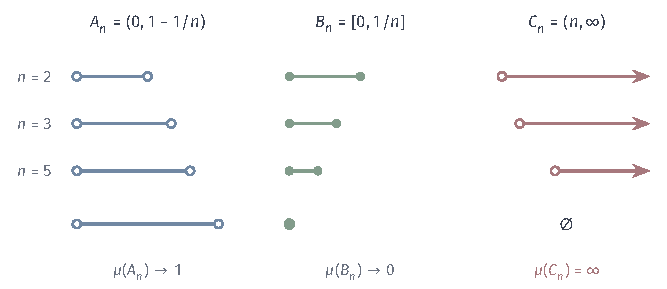
\includegraphics[width=112mm]{figures/00-shared/mathematical-preliminaries-upper/00-shared/tikz/mathematical-language-combinatorics-analysis-optimization-comprehension-additions/nested-set-limits.pdf}
  \caption{实轴上的三列嵌套集合，依次画$n=2,3,5$及最终的并集或交集，均使用勒贝格测度。左列$A_n$递增，并集为$(0,1)$；中列$B_n$递减，交集为$\{0\}$；右列$C_n=(n,\infty)$递减，交集为空，而每一项的测度仍为无穷。空心、实心端点分别表示不包含、包含；各列仅在本列内共用坐标尺度。}
  \label{fig:vol1-add-nested-set-limits}
\end{figure}
\FloatBarrier

\subsubsection{零测集与几乎处处}
\label{sec:comb-null-sets-and-completion}

集合差的测度可以描述遗漏或多出的总量。当这份总量恰为零时，函数仍可能在其中某些点取不同值，某个性质也可能在那里失效。
我们需要说明什么是零测范围、怎样表达一个性质只在零测范围内有例外，以及零测范围究竟能包含多少点。
前两个问题引出零测集和几乎处处，最后一个问题由康托尔集回答；同一删除过程还给出康托尔函数，它的增长全部集中在一个零测集上。

\paragraph{零测集}

测度为零不等于没有元素：勒贝格测度给单点赋值$0$，点本身却仍然存在。
为了用测量值而非点数描述这种范围，先给它一个名称。
\begin{definition}[零测集]
\label{def:analysis-null-set-almost-everywhere}
若$N\in\mathcal L(\mathbb R)$且$m(N)=0$，称$N$为（勒贝格）\term{零测集}（null set）。
\end{definition}
单点与所有可数点集都是零测集：它们是Borel集合，因而可测；由可数次可加性，它们的测度又不超过各单点测度之和$0$。
零测集的任意子集也是零测集：引理~\ref{lem:analysis-zero-outer-measure-measurable}已经证明，外测度为零的集合的子集都可测，单调性又使其测度为零。
因此讨论例外范围时，只要它包含在某个零测集中，就不必再单独验证它的可测性；勒贝格测度的这一性质称为完备性。

\paragraph{几乎处处}

比较两个函数时，除了判断它们是否逐点相等，还可以考察它们取值不同的位置是否都落在一个零测集中。
一般性质的例外范围也用同样的方式描述。
\begin{definition}[几乎处处]
设$E\in\mathcal L(\mathbb R)$。若存在零测集$N$，使某性质对每个$x\in E\setminus N$成立，称该性质在$E$上\term{几乎处处}（almost everywhere，简写为a.e.）成立。
\end{definition}
例如$f(0)=1$、$f(x)=0$（$x\neq0$）与恒零函数几乎处处相等，尽管它们在$0$处并不相等。
例外范围也可以是无限集，并且出现在每一小段中。
\begin{example}[有理点指示函数几乎处处为零]
在$[0,1]$上考虑$f=\mathbb I_{Q_0}$，即$x\in Q_0$时$f(x)=1$，否则$f(x)=0$。
$f$与恒零函数取值不同的点恰好组成$Q_0$，而$m(Q_0)=0$，所以$f=0$在$[0,1]$上几乎处处成立。

再看连续性。$[0,1]$中每个点的任意邻域与$[0,1]$的交都含正长度区间，因而既含$Q_0$中的点，也含无理点；$f$在其中同时取到$1$和$0$，所以$f$在$[0,1]$上处处不连续。
恒零函数则处处连续。
\end{example}

这个例子说明，“几乎处处”不表示只遗漏有限个点，也不表示每个位置附近都没有例外；几乎处处相等也不会自动保留连续性或某个指定点的取值。
后面讨论积分时，会明确哪些结论只依赖零测范围之外的取值。

若一列性质分别在零测集$N_1,N_2,\ldots$之外成立，那么它们在$\bigcup_nN_n$之外同时成立，而这个并仍是零测集。
所以可数多项几乎处处结论可以使用共同的例外范围。这一做法不能推广到不可数多项结论。
\begin{example}[不可数多项几乎处处结论不能合并]
在$[0,1]$上，对每个$t\in[0,1]$考虑性质$P_t$：$x\neq t$。它只在单点$t$处失效，所以每个$P_t$都在$[0,1]$上几乎处处成立。
若要求全部$P_t$同时成立，例外范围是$\bigcup_{t\in[0,1]}\{t\}=[0,1]$，测度为$1$；也就是说，没有任何$x\in[0,1]$满足所有$P_t$。
\end{example}

这里的并有不可数多项，可数次可加性不再适用。

\paragraph{康托尔集}
\label{sec:analysis-cantor-set}

可数集是熟悉的零测集，但零测是否意味着最多只有可数多个点，还需另行检验。
下面的康托尔集说明，点的多少与长度是否为零是两种不同的信息。

记$C_0=[0,1]$。从$C_{n-1}$的每个闭区间中删去中间的开三分之一，得到$C_n$；各层保留集合的交$C=\bigcap_{n\geq0}C_n$称为\term{康托尔集}（Cantor set）。
第$n$层$C_n$由$2^n$个长$3^{-n}$的闭区间组成，总长度为$(2/3)^n$。
按删除规则逐层归纳，这些闭区间恰为$[x_n,x_n+3^{-n}]$，其中$x_n=\sum_{j=1}^nd_j3^{-j}$、$d_j\in\{0,2\}$：从这样的区间删去中间三分之一，留下的两段正对应$d_{n+1}=0$与$d_{n+1}=2$。

下面证明$C$的测度为零，却含不可数多个点。
\begin{example}[康托尔集是不可数零测集]
\label{ex:set-measure-cantor-uncountable-null}
测度：每个$C_n$是有限个闭区间的并，因此$C$是可数个闭集的交，属于Borel集合。
由$C\subseteq C_n$和单调性，$m(C)\leq(2/3)^n$对所有$n$成立，故$m(C)=0$。

点的编码：对每条零一序列$(s_j)_{j\geq1}$，令
\[
 x=\sum_{j=1}^{\infty}\frac{2s_j}{3^j},
\]
即只用数字$0,2$的三进制数。
前$n$位确定的和$x_n=\sum_{j=1}^n2s_j3^{-j}$是$C_n$中某个闭区间的左端点，其余各位之和介于$0$与$\sum_{j>n}2\cdot3^{-j}=3^{-n}$之间，所以$x\in[x_n,x_n+3^{-n}]\subseteq C_n$。
这对每个$n$成立，故$x\in C$。

不同序列给出不同的点：若两条序列首次在第$k$位不同，对应三进制数在该位相差$2\cdot3^{-k}$，其后各位的总差至多$\sum_{j>k}2\cdot3^{-j}=3^{-k}$，所以两点之差至少为$3^{-k}>0$。

零一序列不可数：假定能列出全部序列，把第$n$条序列的第$n$位取反，得到的序列与每条已列序列都至少有一位不同，因而被遗漏。

所以$C$含不可数多个点，是不可数零测集。
\end{example}

零测例外因此能够包含不可数多个点，几乎处处的表述不能用“除去可数多个点”替代。

图~\ref{fig:analysis-process-cantor-deletion}画出上述删除过程：每一步仍有正长度，但总长度$(2/3)^n$随步数趋于零，交集却仍保留点。
\begin{figure}[!htbp]
 \centering
 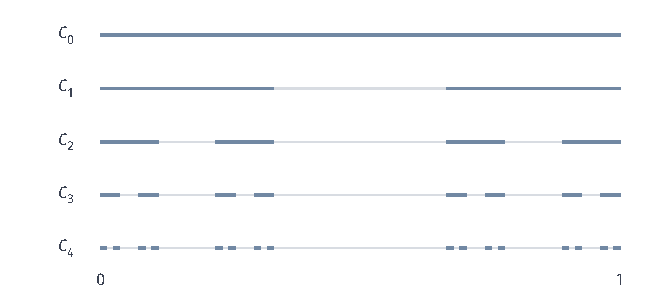
\includegraphics[width=112mm]{figures/00-shared/mathematical-preliminaries-upper/00-shared/tikz/chapter3-concept-processes/cantor-deletion.pdf}
 \caption{蓝线表示$C_0,\ldots,C_4$，每一步从上一行各闭区间中删去中间开三分之一。$C_n$由$2^n$个长度$3^{-n}$的闭区间组成，总长度为$(2/3)^n$；交集$C$的测度因此为零，但始终包含$0,1$。任何有限一行仍有正测度，不能把有限阶段当成最终零测集。}
 \label{fig:analysis-process-cantor-deletion}
\end{figure}

\paragraph{康托尔函数}
\label{sec:analysis-cantor-function}
康托尔集的长度为零，却仍可以承载函数的全部增长。下面用同一删除过程构造一个连续的非减函数：它在每个删去的区间上保持常数，因而在零测集$C$之外导数为零，却从$0$增加到$1$。

$C$中的点在每一步落在左或右保留区间，分别确定三进制表示的下一位为$0$或$2$，所以$C$中每点都有只含这两个数字的表示；示例~\ref{ex:set-measure-cantor-uncountable-null}已说明不同数字序列给出不同的点，因此这种表示唯一。
把三进制数字$0,2$分别改为二进制数字$0,1$，定义
\[
 x=\sum_{j=1}^\infty\frac{\varepsilon_j}{3^j},\qquad
 F(x)=\sum_{j=1}^\infty\frac{\varepsilon_j/2}{2^j},
 \qquad\varepsilon_j\in\{0,2\}.
\]
第二个级数由几何级数$\sum_j2^{-j}$控制，取值在$[0,1]$中；其中$x=1$取全为$2$的表示，$F(1)=1$。

$F$在$C$上不减。若$C$中两点$x<y$的三进制位首次在第$k$位不同，由示例~\ref{ex:set-measure-cantor-uncountable-null}中对首个不同位的估计，较大的$y$在该位取$2$，$x$取$0$。
于是$F(y)$在二进制第$k$位比$F(x)$多$2^{-k}$，而后续各位造成的反向差至多为$\sum_{j>k}2^{-j}=2^{-k}$，所以$F(x)\leq F(y)$。

再把$F$延拓到删去的区间上。若一个开区间在第$k$步删去，它的两端都在$C$中，三进制表示的前$k-1$位相同；左端点第$k$位为$0$而后全为$2$，右端点第$k$位为$2$而后全为$0$。
对应的二进制数分别是该位为$0$而后全为$1$、该位为$1$而后全为$0$，同一个尾和恒等式$\sum_{j>k}2^{-j}=2^{-k}$保证两值相等。
例如$1/3=0.0222\ldots_3$与$2/3=0.2000\ldots_3$都对应$1/2$。
在该开区间上把$F$定义为这个共同值，就得到整个$[0,1]$上的\term{康托尔函数}（Cantor function）。

下面验证康托尔函数的单调性、连续性与导数，并说明它的增长集中在$C$上。
\begin{example}[康托尔函数的连续性与导数]
单调与端点：$F$在$C$上不减，在每个删去区间上取两端的共同值，所以在$[0,1]$上不减，且$F(0)=0$、$F(1)=1$。

一致连续：在第$n$步的每个保留区间上，$C$中的点有相同的前$n$位三进制数字，$F$的值因而有相同的前$n$位二进制数字，都落在一个长$2^{-n}$的区间内；删去区间上的取值也在这个范围中。
所以$F$在每个第$n$步保留区间上的变化不超过$2^{-n}$。
相邻两个第$n$步保留区间之间至少隔着长$3^{-n}$的删去区间，因此两个相距小于$3^{-n}$的点之间至多涉及两个第$n$步保留区间，函数值之差不超过$2^{1-n}$。
对任意给定的误差上界，先选$n$使$2^{1-n}$小于它，再取$\delta=3^{-n}$，就得到一致连续性。

导数：$[0,1]\setminus C$是全部删去开区间的并，$F$在每个删去开区间内恒定，所以$F'=0$于$[0,1]\setminus C$。由于$m(C)=0$，$F'=0$在$[0,1]$上几乎处处成立。

不绝对连续：第$n$步的$2^n$个保留区间总长度为$(2/3)^n\to0$，但每个保留区间两端的$F$值恰好相差$2^{-n}$，端点变化的总和仍为$2^n\cdot2^{-n}=1$。
把定义~\ref{def:measurable-absolutely-continuous-function}中的误差界取为$1$：无论$\delta>0$多小，只要$(2/3)^n<\delta$，这组保留区间的总长度就小于$\delta$，端点变化之和却等于$1$，所以定义的要求不成立。
\end{example}

所以康托尔函数一致连续（因而连续）、几乎处处导数为零，全部增长$F(1)-F(0)=1$却集中在零测集$C$上。
第~\ref{sec:analysis-fundamental-calculus}节将用它说明，只知道函数连续且几乎处处可导，不能由导数的积分恢复端点变化。

\FloatBarrier
